\subsection{Casa Familia}

\begin{figure}[H]
	\center
	\begin{subfigure}{0.4\textwidth}
		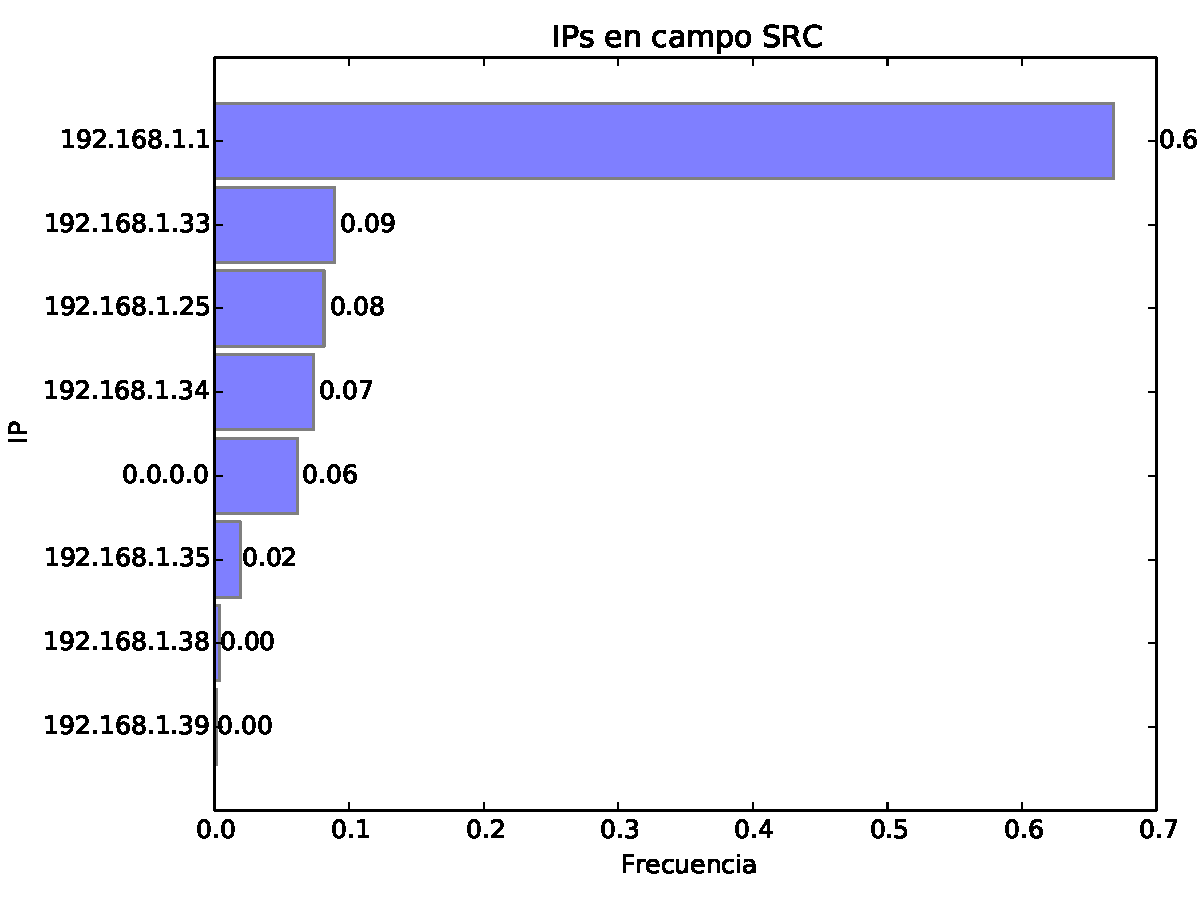
\includegraphics[width=1.0\textwidth]{resultados/casa/ipsSrc_1_6805902069.pdf}
		\caption{Estimaci\'on de la probabilidad de cada s\'imbolo en modelo SRC}
	\end{subfigure}
	~
	\begin{subfigure}{0.4\textwidth}
		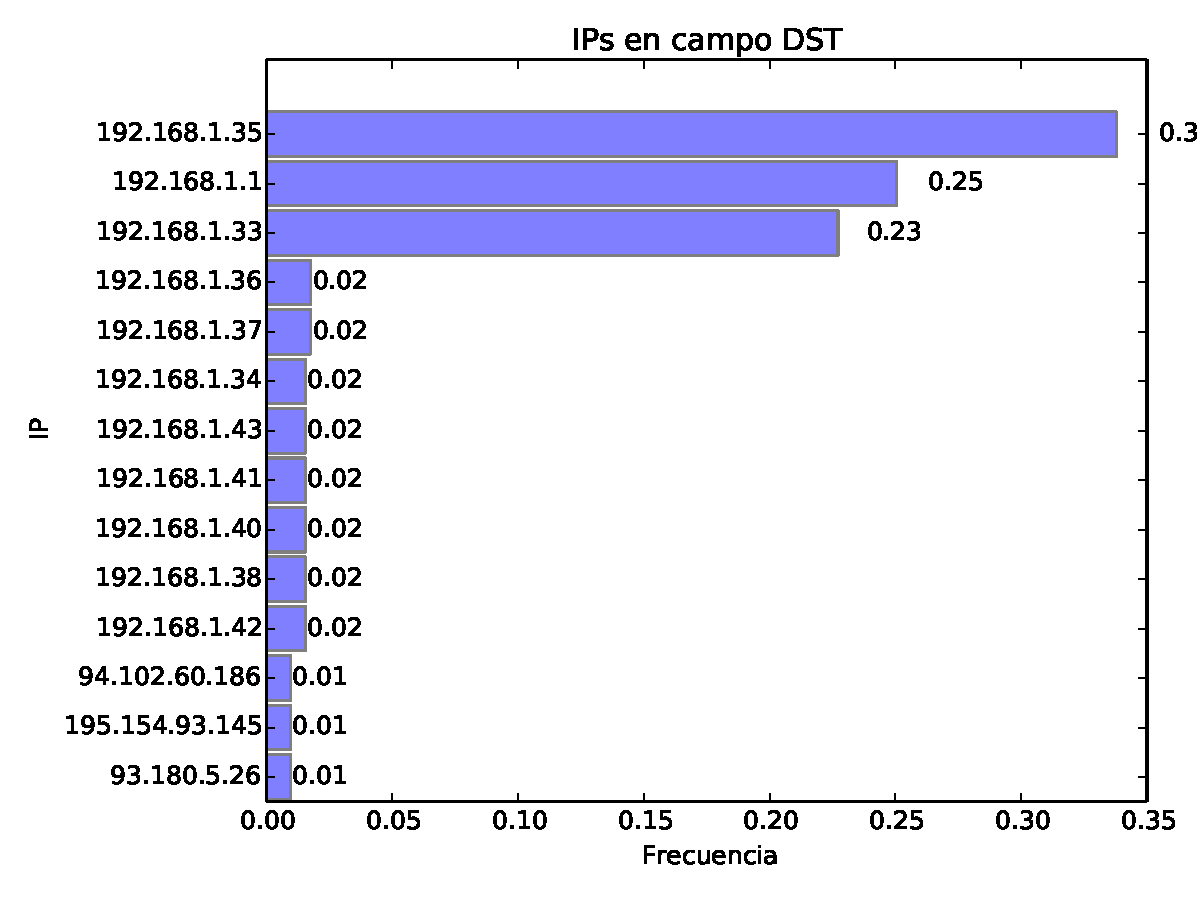
\includegraphics[width=1.0\textwidth]{resultados/casa/ipsDst_2_67355481854.pdf}
		\caption{Estimaci\'on de la probabilidad de cada s\'imbolo en modelo DST}
	\end{subfigure}
\end{figure}

\begin{wrapfigure}{R}{0.4\textwidth}
\vspace{-35pt}
\hspace{-35pt}
\centering
   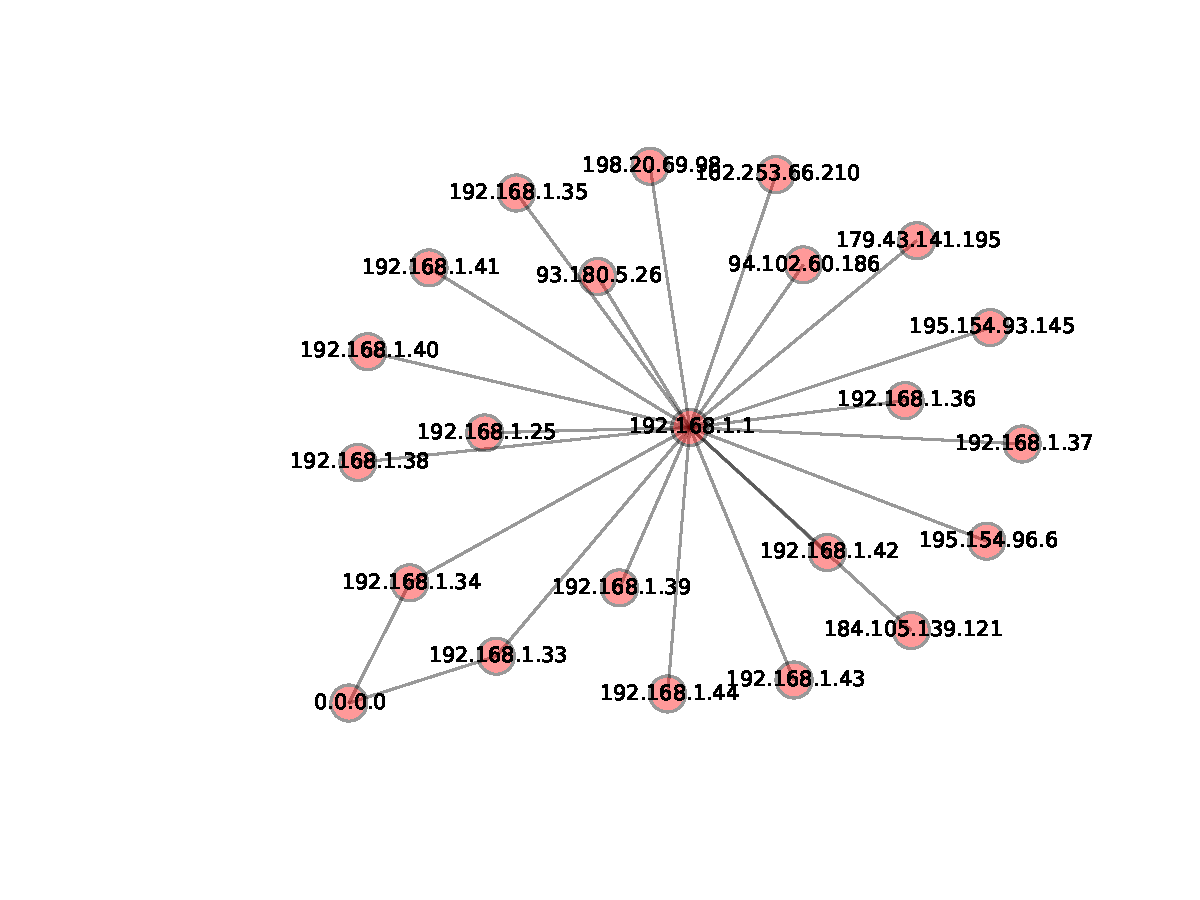
\includegraphics[width=0.4\textwidth]{resultados/casa/conectividadNX.pdf}
\vspace{-30pt}
   \caption{Grafo de la red}
\end{wrapfigure}

En el caso de la casa familiar sabiamos de antemano que el router es 192.168.1.1. Dicha ip es de las
que aparecen con mayor frecuencia en los campos SRC o DST. Ambos grafos presentan forma de estrella,
teniendo al router como centro. La entrop\'ia fue: $1.68$ para el modelo $SRC$ y $2.67$ para el modelo
DST. Cabe destacar que aunque no est\'a reflejado en los gr\'aficos, sucedi\'o algo interesante, 
aparecieron paquetes ARP con direcciones que no pertenecian a la red local, esto se puede deber a que
 \textcolor{red}{NO TENGO LA MENOR IDEA}





\begin{figure}[H]
   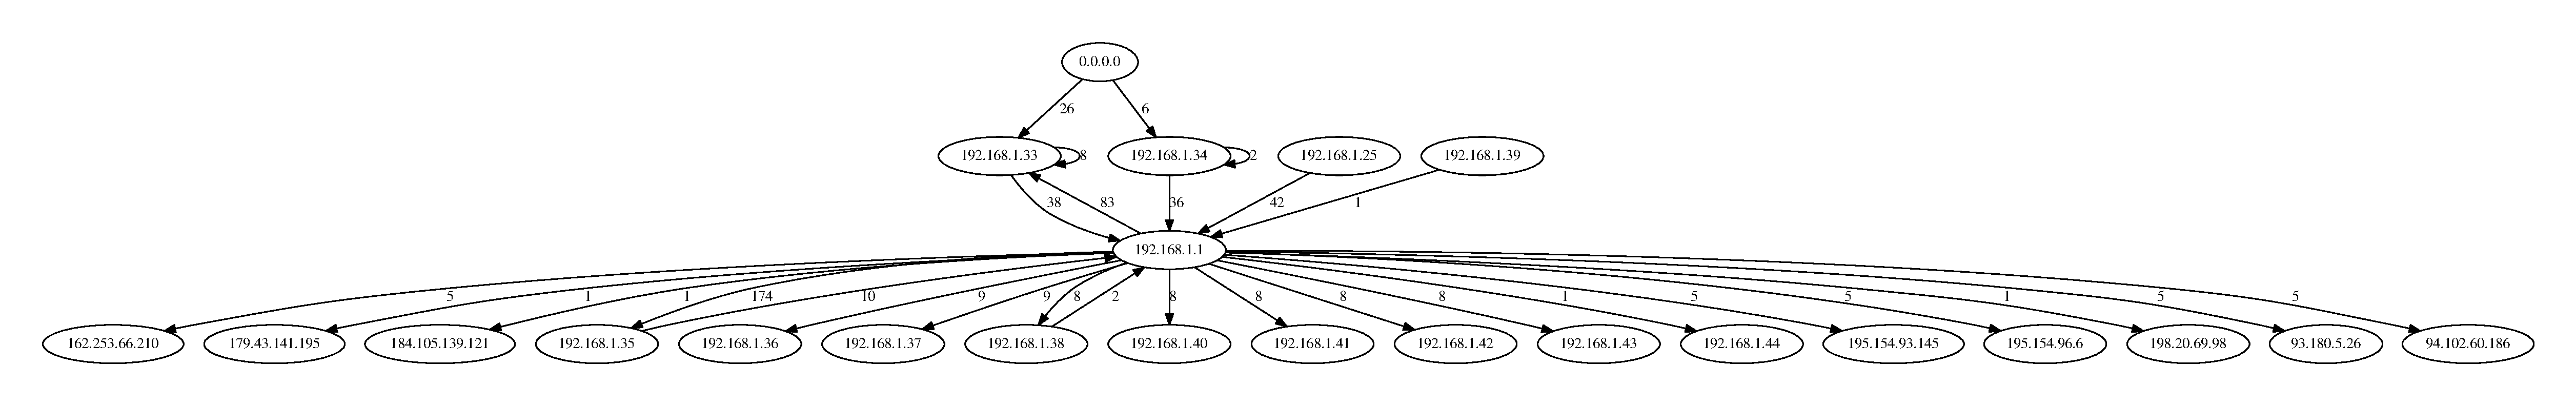
\includegraphics[width=1.0\textwidth]{resultados/casa/conectividad.pdf}
   \caption{Grafo dirigido de la red con peso en las aristas}
\end{figure}





